\documentclass[../main.tex]{subfiles}
\begin{document}
\section{映射}
\begin{definition}[映射]\label{def:II.1.3}
    设$X$和$Y$是集合,如果由$X$到$Y$的关系$f$同时满足:
    \begin{enumerate}
        \item $\mathrm{dom}f=X$;
        \item 对每一$X$的元素$x\in X$,\emph{有且只有一个}$Y$的元素$y\in Y$满足$\left(x,y\right)\in f$,
    \end{enumerate}
    则称$f$是由$X$到$Y$的\emph{映射(mapping)},记作$f:X\rightarrow Y$\footnote{记号$f:X\rightarrow Y$包含的信息是:
        \begin{enumerate}
            \item $X$、$Y$是集合;
            \item $f$是由$X$到$Y$的映射。
        \end{enumerate}
    }。对每一$\left(x,y\right)\in f$,称$y$是$x$在映射$f$下的\emph{值(value)},记作$f\left(x\right)$。
\end{definition}

\begin{figure}[htbp]
    \centering
    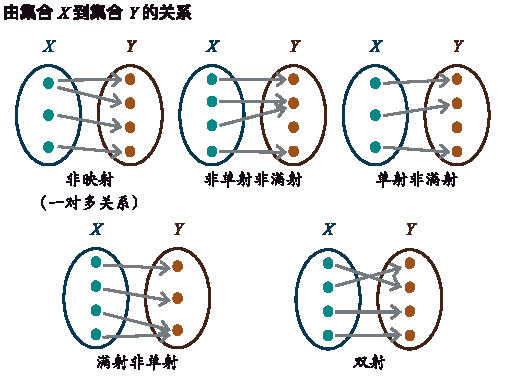
\includegraphics{../images/mapping.pdf}
    \caption{映射的不同概念示意图。}
    \label{fig:II.1.3}
\end{figure}

映射定义的第1条要求如果违反了,可通过对集合$X$的改动重新得到满足,而无需改动关系$f$本身。例如若$\mathrm{dom}f\subsetneqq X$,则令$X^\prime=\mathrm{dom}f$并改为讨论由$X^\prime$到$Y$的关系$f$,就可通过映射定义的第1条。然而映射定义的第2条如果违反了,想要重新满足就不得不对关系$f$本身进行改动。图\ref{fig:II.1.3}中的第一个例子就只是一个关系,而不是一个映射,除非我们从这一关系中拿掉一个有序对。

给定映射$f:X\rightarrow Y$,我们继续以下讨论:
\begin{itemize}
    \item 一般地,$Y$未必等于$\mathrm{ran}f$,集合$Y$称映射$f$的\emph{陪域(codomain)}。
    \item 若$E$是$X$的一个子集,若由$E$到$Y$的映射$\left.f\right|_E:E\rightarrow Y$满足$\left.f\right|_A\left(x\right)=f\left(x\right),\forall x\in E$,则称映射$\left.f\right|_E$是映射$f$在$E$上的\emph{限制(restriction)}(记法亦已表明)\footnote{通俗说$f$在$A$上的限制跟$f$是同一个映射,只不过定义在了“更小的”一个集合$A$上罢了。}。
    \item 若$\mathrm{ran}f=Y$则称映射$f$是\emph{满射(surjective mapping)}。图\ref{fig:II.1.3}中的第4和第5个例子都是满射。
    \item 若$A\subset X$,则集合$\left\{y\in Y|\forall x\left(x\in A\wedge y=f\left(x\right)\right)\right\}$称集合$A$在映射$f$下的\emph{像(image)},简记为$f\left(A\right)$。这一集合可用语言描述为:由集合$A$的所有元素在映射$f$下的值组成的集合。易证它是$Y$的子集。
    \item 若对任意$x_1,x_2\in X$,$f\left(x_1\right)=f\left(x_2\right)\Rightarrow x_1=x_2$,则称$f$是\emph{单射(injective mapping)}。可用语言描述为,“单射的输出唯一地确定其输入”。图\ref{fig:II.1.3}中的第3和第5个例子都是单射。
    \item 如果$f$既是满射又是单射,则称$f$是一个\emph{双射(bijective mapping)}。图\ref{fig:II.1.3}中的第5个例子是双射。
    \item 若另一映射$g:Y\rightarrow Z$,可与映射$f$构成从$X$到$Z$的映射$g\circ f:X\rightarrow Z$,且
          \[
              g\circ f\left(x\right)=g\left(f\left(x\right)\right),\forall x\in X
          \]
          则称$g\circ f$是$f$和$g$的\emph{复合映射(composite mapping)}。
    \item 如果$f\left(x\right)=x,\forall x\in X$,则称映射$f$是\emph{恒等映射(identity mapping)}。
    \item 如果映射$g:Y\rightarrow X$使得复合映射$g\circ f$是恒等映射,则称映射$f$是\emph{可逆的(invertible)},映射$g$是$f$的\emph{逆映射(inverse mapping)}。常将$f$的逆映射记作$f^{-1}$。
\end{itemize}

关于逆映射,有一条重要的定理——

\begin{theorem}\label{thm:II.1.2}
    双射必存在唯一逆映射。双射的逆映射也是双射。
\end{theorem}
\begin{proof}
    为了证明这一定理,我们首先证明一个引理:任一单射非满射均存在逆映射。

    设$f:X\rightarrow Y$是一个单射非满射,即$\exists y\notin\mathrm{ran}f,y\in Y$。由集合的相关定义此处必有$\left\{y|y\in\mathrm{ran}f\right\}\cup\left\{y|y\notin\mathrm{ran}f,y\in Y\right\}=Y$。

    现定义$g:Y\rightarrow X$,为使$g$为一个映射,它必须对$y\in\mathrm{ran}f$和$y\notin\mathrm{ran}f,y\in Y$均有定义。现将其定义为:
    \[
        g\left(y\right)=\left\{
        \begin{array}{ll}
            \left.x\right|_{f\left(x\right)=y}, & y\in\mathrm{ran}f           \\
            \text{任一}x\in X,                    & y\notin\mathrm{ran}f,y\in Y
        \end{array}
        \right.
    \]
    则有如下几条结论:
    \begin{enumerate}
        \item $g\left(y\right)$是映射。因为它对每一$y\in Y$均有定义且一个$y\in Y$只对应一个$x\in X$。
        \item $g$是满射。因为,仅$y\in\mathrm{ran}f$情况的定义式就已决定了$\mathrm{ran}g=X$。
        \item $g$是非单射。因为$g$是满射,再考虑$y\notin\mathrm{ran}f,y\in Y$情况的定义式,就可知$\exists x\in X$满足$x=g\left(y\right)=g\left(y^\prime\right)$,其中$y\neq y^\prime,y\in\mathrm{ran}f,y^\prime\notin\mathrm{ran}f,y^\prime\in Y$。
        \item $g$是$f$的逆映射。因为,对于任一$x\in X$均有$g\circ f\left(x\right)\equiv g\left(f\left(x\right)\right)=x$,即$g\circ f=\mathrm{id}_X$。
        \item 一般地,$g$是不唯一的。因为$y\notin\mathrm{f},y\in Y$的情况可定义$g\left(x\right)$等于任一$x\in X$,故只要集合$X$不是只有一个元素,那么$g$都不唯一。
    \end{enumerate}
    该引理证毕。

    现在正式证定理\ref{thm:II.1.2}。从上面定义的这个$g$继续,如果$g$是双射,则$g$不仅是满射,还是单射。由刚刚证完的引理,可用类似方法给$g$找一个逆映射$f^\prime:X\rightarrow Y$。而且,由于$\mathrm{ran}g\equiv X$,我们无需像定义$g$那样为$f^\prime$分出$x\notin\mathrm{ran}g,x\in X$的情况,因为不存在这种情况。故
    \[
        f^\prime\left(x\right)=\left.y\right|_{g\left(y\right)=x}
    \]
    是$g$的逆映射,且$f^\prime$是满射。而且,把$g$的定义代入上式有$f^\prime\left(x\right)=\left.y\right|_{g\left(y\right)=x}=\left.y\right|_{\left.x\right|_{f\left(x\right)=y}}=f\left(x\right)$,即$f^\prime$不是别的映射而恰为$f\left(x\right)$。即$g$的逆映射是唯一的。因$f^\prime$是满射故$f$是满射,而$f$本身就是单射,故$f$是双射。
\end{proof}

% 需要增加“族”的概念。这至少是多于2个集合的笛卡尔积的基础。
我们常把映射写成另一种形式,并给以另一个名称。具体地,当我们把由$I$到$X$的映射$x:I\rightarrow X$改称为\emph{索引族(indexed family)}时,定义域$I$就称为\emph{索引集(indexing set)},其元素$i\in I$称为\emph{索引(indexes)}。映射$x$的关于$i\in I$的值,记作$x_i$,称为该索引族的一\emph{项(term)}。映射$x$的值域,称作\emph{由$I$索引的集合(set indexed by $I$)},或笼统地称其为一个\emph{索引集(indexed set)}。我们经常不加分辨地直接把$\left\{x_i\right\}_{i\in I}$称为一个\emph{由$I$索引的族($I$-indexed family)}。可见,我们无非把映射原有概念的名称换了一套新的名称。我们经常讨论的是以集合为项的族,称为\emph{集合的索引族(indexed family of sets)}。

设$\mathcal{C}$是集合的集合。如果有$\mathcal{C}$恰好还是一个由集合$I$索引的集合,$\mathcal{C}=\left\{X_i\right\}_{i\in I}$,那么第一节介绍的$\mathcal{C}$的元素的交集和并集就相应有新的表示方式:
\[
    \bigcap_{X\in\mathcal{C}}X=\bigcap_{i\in I}X_i,\quad\bigcup_{X\in\mathcal{C}}X=\bigcup_{i\in I}X_i
\]

下面我们介绍多于两个集合的笛卡尔集的定义\footnote{第一节中引入的两个集合的笛卡尔集定义,无法推广至不可数无穷多个集合间的笛卡尔积。所以,我们在介绍了映射之后,在族的基础上可重新定义笛卡尔集。这个新的定义,在集合个数为两个的情况下,也导致一种与老定义不同的“有序对”,但是新定义和老定义得出有序对之间总是一一对应的,因此无所谓从哪种定义去理解有序对。虽然笛卡尔积的新定义既兼容两个集合间的情况(甚至把“一个集合的笛卡尔集”也定义了),又能够推广到不可数无穷个集合间的笛卡尔集,但是它却不能在一开始就采用,因为它依赖映射的定义,而映射是一种关系,关系的定义依赖有序对的定义。所以我们至少需要先以老定义获得有序对的概念,才能走到现在这一步。}

\begin{definition}[笛卡尔积]\label{def:Cartesian_product_family}
    设$\left\{S_i\right\}_{i\in I}$是由$I$索引的族,且它是集合的索引族,$\left\{s_i\right\}_{i\in I}$也是由$I$索引的族,且$s_i\in S_i,\forall i\in I$。我们称$\left\{S_i\right\}_{i\in I}$的笛卡尔积是由$\left\{S_i\right\}_{i\in I}$得出的所有族$\left\{s_i\right\}_{i\in I}$的集合,记为
    \[
        \prod_{i\in I}S_i
    \]
    若$S_i=S,\forall i\in I$,则记$\prod_{i\in I}S_i\equiv S^I$。
\end{definition}


% 这个例子的功能是让读者理解这个定义。因此需要更加step-by-step,也许要使用图形。
\begin{example}
    设$I=\left\{a,b\right\},X_a=\left\{a_\alpha,a_\beta\right\},X_b=\left\{b_\alpha,b_\beta\right\}$,则按照笛卡尔积的老定义,
    \[
        X_a\times X_b=\left\{\left(a_\alpha,b_\alpha\right),\left(a_\alpha,b_\beta\right),\left(a_\beta,b_\alpha\right),\left(a_\beta,b_\beta\right)\right\}
    \]
    其中按照有序对的老定义,$\left(x,y\right)=\left\{\left\{x\right\},\left\{x,y\right\}\right\}$。

    按照新定义\ref{def:Cartesian_product_family}的要求,我们要在$X_a$和$X_b$中各选一个元素组成由$\left\{a,b\right\}$索引的族$\left\{x_i\right\}_{i\in\left\{a,b\right\}}$。例如,令$x_a=a_\beta,x_b=b_\alpha$所形成的族$\left\{x_i\right\}_{i\in\left\{a,b\right\}}\equiv\left\{x_a,x_b\right\}=\left\{a_\beta,b_\alpha\right\}$就是其中一个符合要求的族。所有这样的族,一共有4个。因此有
    \[
        \prod_{i\in\left\{a,b\right\}}X_i=\left\{\left\{a_\alpha,b_\alpha\right\},\left\{a_\alpha,b_\beta\right\},\left\{a_\beta,b_\alpha\right\},\left\{a_\beta,b_\beta\right\}\right\}
    \]
\end{example}

% 这里要加一段设问:
% 1. 为啥要新定义?
% 2. 新定义和老定义得出的东西是不一样的。那老定义怎么办?
% 3. 为什么不一开始就按新定义?
% 4. 新老定义总是要同时写在书上。
% 5. 那在同一文本中,同一概念新老定义会冲突?
% 6. 在二元的情况下两个定义得到的东西虽然不一样,但是元素一一对应。因此不造成问题。

笛卡尔积的老定义与新定义是不冲突的。一般地,老定义下的笛卡尔积$X_a\times X_b$和新定义下的笛卡尔集$\prod_{i\in\left\{a,b\right\}}X_i$之间总可以定义一个映射$f:\prod_{i\in\left\{a,b\right\}}X_i\rightarrow X_a\times X_b,f\left(z\right)=\left(z_a,z_b\right),\forall z\equiv\left\{z_i\right\}_{i\in\left\{a,b\right\}}\in\prod_{i\in I}X_i$。记$z=\left\{z_i\right\}_{i\in\left\{a,b\right\}}$,则按定义\ref{def:Cartesian_product_family}有$z_i\in X_i,\forall i\in\left\{a,b\right\}$。可以证明$f$是双射:
\begin{proof}
    设$z=\left\{z_i\right\}_{i\in\left\{a,b\right\}},z^\prime=\left\{z^\prime_i\right\}_{i\in\left\{a,b\right\}}$且$z_a,z^\prime_a\in X_a,z_b,z^\prime_b\in X_b$。若$z\neq z^\prime$。由映射$f$的定义,$f\left(z\right)=\left(z_a,z_b\right),f\left(z^\prime\right)=\left(z^\prime_a,z^\prime_b\right)$。由集合相等的定义,$z\neq z^\prime\Rightarrow\left(z_a,z_B\right)\neq\left(z^\prime_a,z^\prime_b\right)$,即$f\left(z\right)\neq f\left(z^\prime\right)$,即$f$是非单射。

    设$\left(u,v\right)\in X_a\times X_b$\footnote{此处我们需要规定,只要集合$X$和$Y$都是非空集合,那么它们的笛卡尔集$X\times Y$也是非空集合,即必存在一$\left(x,y\right)\in X\times Y,x\in X,y\in Y$。这是集合论的\emph{选择公理(axiom of choice)}。},则以$\left\{a,b\right\}$索引的族$x\equiv\left\{x_i\right\}_{i\in\left\{a,b\right\}},x_a=u,x_b=v$满足$x_a\in X_a,x_b\in X_b$(按照笛卡尔积的老定义),按照定义\ref{def:Cartesian_product_family},有$x\in\mathrm{dom}f$。由于所选取的$X_a\times X_b$的元素$\left(u,v\right)$是任意的,上述性质对任一$X_a\times X_b$的元素都成立,故$f$是满射。

    由双射的定义,$f$是双射。
\end{proof}

% 以下需要讨论的是:
% 1. 我们从此以后就只用新定义。
% 2. 这将限制了允许我们进行笛卡尔积的情况。当我们无法为我们想要作的笛卡积设计一个映射把所要作笛卡尔积的集合转化成它们的簇,那么我们在数学上就不被允许作这种笛卡尔积,或说这样的笛卡尔积没有意义。所幸的是,这样的情况很难想象(以作者有限的知识,还未见关于这种情况不存在的证明)。
% 应该举几种例子。一是:一个一集合的集合上的笛卡尔积;几个集合之间,有重复的笛卡尔焦;X^R;……

因此,笛卡尔集的新定义\ref{def:Cartesian_product_family}在集合数为2的情况下所得到的集合,跟笛卡尔集的老定义所得到的集合,它们的元素之间是一一对应的。在此情况下老定义和新定义没有本质差别。根据笛卡尔积的新定义,“有序对”又可以定义成索引集有两个元素的族。即$\left(x,y\right)=\left\{z_i\right\}_{i\in\left\{a,b\right\}},z_a=x,z_b=y$。这时“序”的性质仍被保留,因为$\left(y,x\right)=\left\{z_i\right\}_{i\in\left\{a,b\right\}},z_a=y,z_b=x$是不同的族,故有$\left(x,y\right)\neq\left(y,x\right)$。而且,按照新定义,仅通过改变索引集元素的个数,就可方便地推广出“有序三元组”、“有序四元组”……的定义,这是比老定义更有利的地方。从今以后,笛卡尔积就不再采用老定义,而采用定义\ref{def:Cartesian_product_family}。就算若干个两两不同的集合$X,Y,\cdots$尚未成为一个索引族,由于易验任一集合的非空集合$\mathcal{C}$均可充当其自己的索引集而成为一个索引族,故由$X,Y,\cdots$组成的集合$\left\{X,Y,\cdots\right\}$总能成为一个索引族,从而它们的笛卡尔集仍可通过定义\ref{def:Cartesian_product_family}得到定义。更一般地,给定任一集合的集合$\mathcal{C}$,若$\mathcal{C}\neq\emptyset$,则它的元素的笛卡尔积可由定义\ref{def:Cartesian_product_family}记为
\[
    \prod_{X\in\mathcal{C}}X\equiv\prod_{i\in\mathcal{C}}A_i,\quad A_i=i,\forall i\in\mathcal{C}
\]

我们常讨论索引集$I$为自然数集$\mathbb{N}$的子集\footnote{本讲义默认读者常识上理解各种数集,而不再介绍它们的集合论引入。}的族,即$I\subset\mathbb{N}$。具体地,若
\[I=\left\{a,a+1,a+2,\cdots,b-2,b-1,b\right\},a,b\in\mathbb{N},a<b\]则由$I$索引的族可记为$\left\{X_i\right\}_{i=a}^b$。相应地,若该族是集合的族,则该族的交集、并集和笛卡尔积可分别记为:
\[
    \bigcap_{i=a}^b X_i,\quad\bigcup_{i=a}^b X_i,\quad\prod_{i=a}^b X_i
\]
特别地,若$X_i=X,\forall i\in I$,令$n=b-a+1$,$\left\{X_i\right\}_{i=a}^b$的笛卡尔积可记为$X^n$。例如,$\mathbb{R}^n$是所有有序实数$n$元组$\left(x_1,\cdots,x_n\right),x_1,\cdots,x_n\in\mathbb{R}$的集合。在数学中我们常常会称$\mathbb{R}^n$是“$n$维”的。因此,定义\ref{def:Cartesian_product_family}的好处是它可以支持各种无穷维空间的构造。
\end{document}